\documentclass[a4paper,12pt]{book}
\usepackage[utf8]{inputenc}
\usepackage{graphicx}
\usepackage{caption}
\usepackage{subcaption}
\graphicspath{ {./screen_shots/} }
\usepackage{hyperref}

\begin{document}

\author{}
\title{MANUAL v0.14}
\date{25 June 2023}

\frontmatter
\maketitle
\tableofcontents

\mainmatter

\chapter{Introduction}
This manual v0.14 is prepared for mobile mapping system \href{https://github.com/JanuszBedkowski/mandeye_controller/blob/main/doc/manual/manual_v0_1/mandeye_dev_manual_v0_1.pdf}{MANDEYE} available as open hardware project.
The software is composed of:
\begin{itemize}
	\item Lidar odometry (for initial trajectory calculation),
	\item Multi view terrestrial laser scan registration (for final trajectory calculation).
\end{itemize}


\chapter{Lidar odometry}
This software calculates trajectory based on Lidar and IMU data.
It based on novel approach that I did not have opportunity to publish (work in progress).
Basically it is SAM (Smoothing and Mapping) approach that is using multi view Normal Distributions Transform in pose graph SLAM framework writen from scratch in Python (SymPy) and C++ (Eigen).
 

\begin{figure}
	\centering
	\includegraphics[width=\textwidth]{1.png}
	\caption{Step 1 - loading data.}
	\label{fig:1}
\end{figure}

\begin{figure}
	\centering
	\includegraphics[width=\textwidth]{2.png}
	\caption{Step 2 - select all *.csv and *.laz files from folder that \href{https://github.com/JanuszBedkowski/mandeye_controller/blob/main/doc/manual/manual_v0_1/mandeye_dev_manual_v0_1.pdf}{MANDEYE} mobile mapping system created on USB drive.}
	\label{fig:2}
\end{figure}

\begin{figure}
	\centering
	\includegraphics[width=\textwidth]{3.png}
	\caption{Step 3 - press 'compute all'. Check console mean time and folder 'preview'.}
	\label{fig:3}
\end{figure}

\begin{figure}
	\centering
	\includegraphics[width=\textwidth]{4.png}
	\caption{Optional step: intermediate results are stored in 'preview' folder.}
	\label{fig:4}
\end{figure}

\begin{figure}
	\centering
	\includegraphics[width=\textwidth]{5.png}
	\caption{Optional step: You can watch the progress in open source \href{https://www.cloudcompare.org/}{CloudCompare} software by loading all *.laz files from 'preview' folder.}
	\label{fig:5}
\end{figure}

\begin{figure}
	\centering
	\includegraphics[width=\textwidth]{6.png}
	\caption{Progress in console.}
	\label{fig:6}
\end{figure}

\begin{figure}
	\centering
	\includegraphics[width=\textwidth]{7.png}
	\caption{Final data in \href{https://www.cloudcompare.org/}{CloudCompare}.}
	\label{fig:7}
\end{figure}

\begin{figure}
	\centering
	\includegraphics[width=\textwidth]{8.png}
	\caption{Final data ready for export.}
	\label{fig:8}
\end{figure}

\begin{figure}
	\centering
	\includegraphics[width=\textwidth]{9.png}
	\caption{Exported final files.}
	\label{fig:9}
\end{figure}

\chapter{Multi view terrestrial laser scan registration (steps 2 and 3)}
\section{Step 2}
\begin{figure}[H]
	\centering
	\includegraphics[width=\textwidth]{10.png}
	\caption{Load session.json prepared by 'Lidar odometry'.}
	\label{fig:10}
\end{figure}

\begin{figure}[H]
	\centering
	\includegraphics[width=\textwidth]{13.png}
	\caption{Prepare field of view and change decimation to see more points. Generate random colors option is recommended for next steps as every scan will be in a different color.}
	\label{fig:13}
\end{figure}

\begin{figure}[H]
	\centering
	\includegraphics[width=\textwidth]{14.png}
	\caption{Turn on Manual Pose Graph Loop Closure Mod, then choose two different scans that share scanned objects, but difference in their numbers is as big as possible e.g. when you made a loop during scanning and came back to the same place after some time. Then click add edge.} 
	\label{fig:14}
\end{figure}

\begin{figure}[H]
	\centering
	\includegraphics[width=\textwidth]{15.png}
	\caption{Turn on manipulate active edge, turn on gizmo and align scan to scan manually.}
	\label{fig:15}
\end{figure}

\begin{figure}[H]
	\centering
	\includegraphics[width=\textwidth]{16.png}
	\caption{Once You are not capable align more accurate, then turn off gizmo and repetitively use ICP until scans align to the level at which nothing can change anymore.}
	\label{fig:16}
\end{figure}

\begin{figure}[H]
	\centering
	\includegraphics[width=\textwidth]{17.png}
	\caption{Turn off manipulate active edge, click "set initial poses as motion model", then click "compute pose graph SLAM".}
	\label{fig:17}
\end{figure}

\begin{figure}[H]
	\centering
	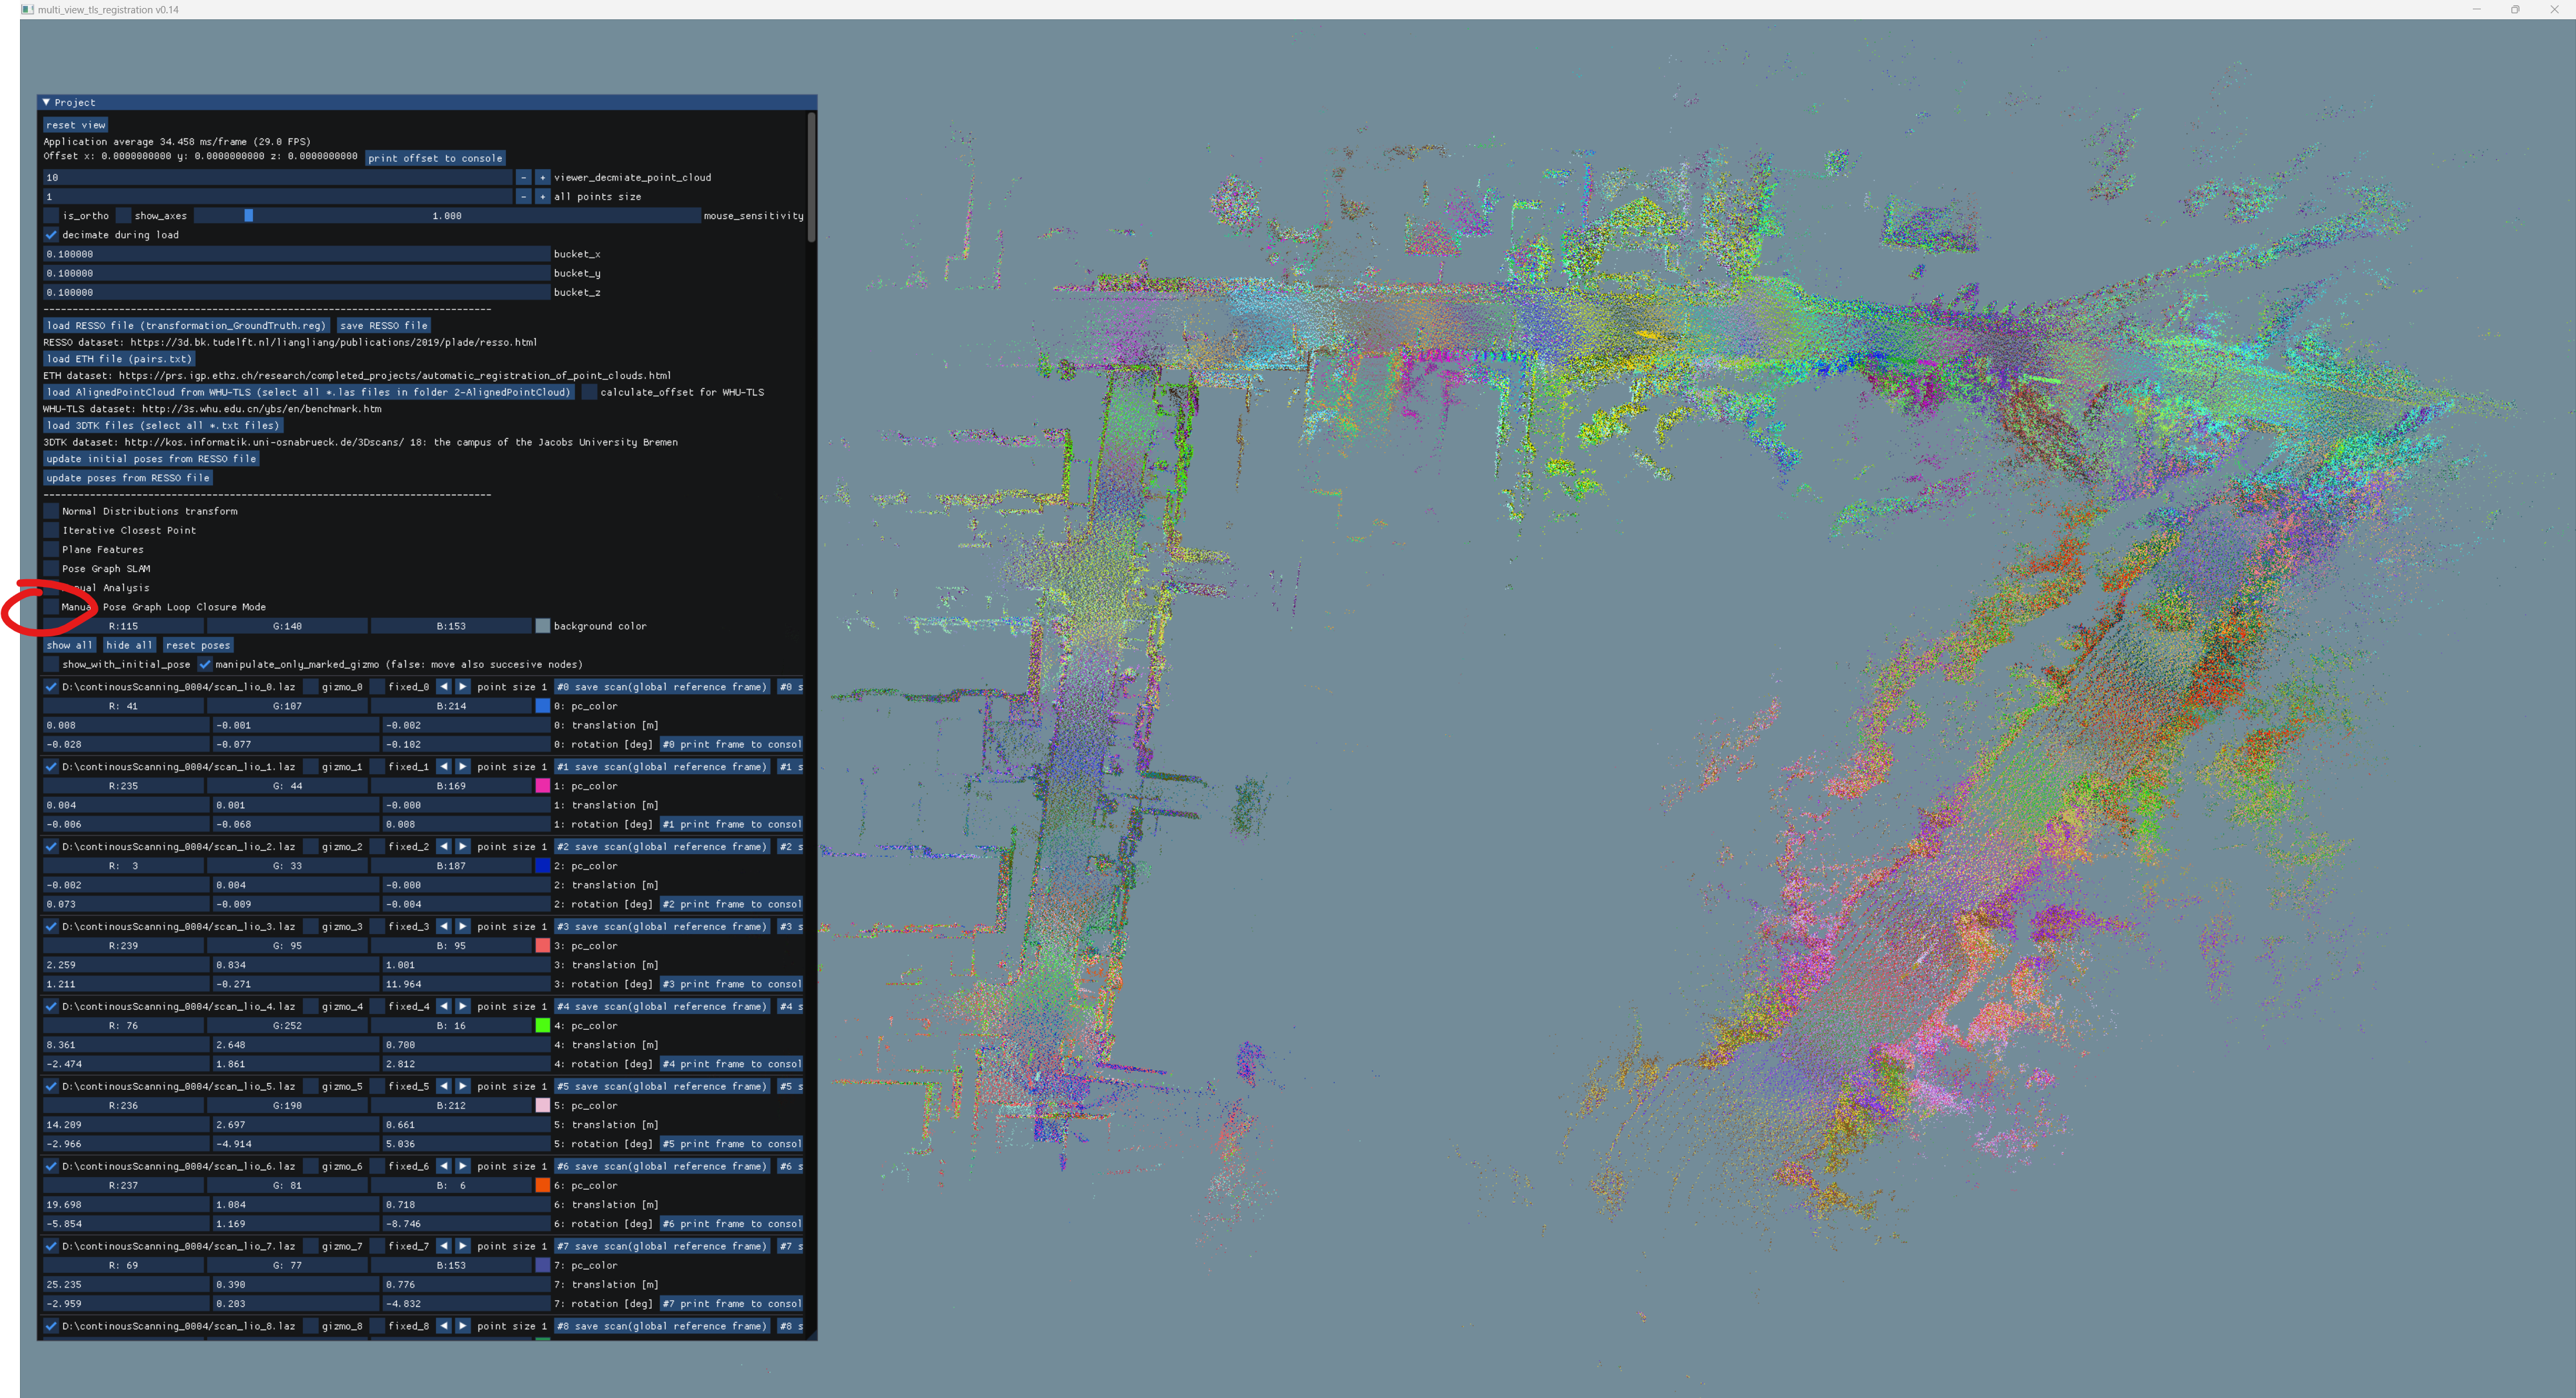
\includegraphics[width=\textwidth]{18.png}
	\caption{Turn off Manual Pose Graph Loop Closure Mod and inspect if everything is ok, if not,  repeat steps from figures 3.3-3.6 (choose another pair of scans, refine them and compute the pose graph SLAM).}
	\label{fig:18}
\end{figure}

\begin{figure}[H]
	\centering
	\includegraphics[width=\textwidth]{19.png}
	\caption{Once the job is done click Save session button to save changes to session.json and export data to *.laz. The latter is Your map that can be loaded by e.g. \href{https://www.cloudcompare.org/}{CloudCompare}.}
	\label{fig:19}
\end{figure}

\section{Step 3}
\begin{figure}[H]
	\centering
	\includegraphics[width=\textwidth]{20.png}
	\caption{Add sessions that you want to align.}
	\label{fig:20}
\end{figure}

\begin{figure}[H]
	\centering
	\includegraphics[width=\textwidth]{21.png}
	\caption{Choose session.json files - effects of the lidar odometry step.}
	\label{fig:21}
\end{figure}

\begin{figure}[H]
	\centering
	\includegraphics[width=\textwidth]{22.png}
	\caption{Click load sessions button and wait for the chosen sessions to load.}
	\label{fig:22}
\end{figure}

\begin{figure}[H]
	\centering
	\includegraphics[width=\textwidth]{23.png}
	\caption{When all of the sessions have loaded activate Manual Pose Graph Loop Closure Mode. If more than 2 sessions were loaded, deactivate sessions till two of them remain. After that the button should appear.}
	\label{fig:23}
\end{figure}

\begin{figure}[H]
	\centering
	\includegraphics[width=\textwidth]{24.png}
	\caption{Choose 2 individual scans of the same area, one from the first session, other from the second session and click add edge.}
	\label{fig:24}
\end{figure}

\begin{figure}[H]
	\centering
	\includegraphics[width=\textwidth]{25.png}
	\caption{Click manipulate active edge, then gizmo and as in \hyperref[fig:15]{the step 2} align scans as precisely as possible and then repeatedly use ICP till nothing changes.}
	\label{fig:25}
\end{figure}

\begin{figure}[H]
	\centering
	\includegraphics[width=\textwidth]{26.png}
	\caption{After aligning scans turn off Manual Pose Graph Loop Closure Mode, click Optimize and if everything is ok then click Save results. Should anything go wrong and sessions haven't orientated as planned just use Revert button. Repeat steps 3.13-3.15 until two sessions are aligned with a satisfying effect.}
	\label{fig:26}
\end{figure}

\begin{figure}[H]
	\centering
	\includegraphics[width=\textwidth]{27.png}
	\caption{At the end or in the middle of work you can save your project to .json file, which can be loaded next time multi session registration step 3 is used.}
	\label{fig:27}
\end{figure}

\backmatter
% bibliography, glossary and index would go here.

\end{document}